%%%%%%%%%%%%%%%%%%%%%%%%%%%%%%%%%%%%    
%%%%%%%%%%%%%%%%%%%%%%%%%%%%%%%%%%%%%%%%%%%%
% Preamble                                                                     %
%%%%%%%%%%%%%%%%%%%%%%%%%%%%%%%%%%%%%%%%%%%%%%%%%%%%%%%%%%%%%%%%%%%%%%%%%%%%%%%%

\documentclass[a4paper,spanish,10p,titlepage]{report}

\usepackage[utf8]{inputenc}
\usepackage{estilo_pfc}

\author{Pablo Castro Valiño}
\date{14 de xaneiro de 2016}

%% Para eliminar as todonotes do texto, engade ás propiedaes da
%% documentclass o atributo "final".
\usepackage[obeyFinal]{todonotes}
\newcommand{\santiagosays}[2][inline]{\todo[author=Santiago,color=yellow,#1]{#2}}
\newcommand{\ProTip}[2][inline]{\todo[author={\bf ProTip}™,color=cyan,#1]{#2}}

%%%%%%%%%%%%%%%%%%%%%%%%%%%%%%%%%%%%%%%%%%%%%%%%%%%%%%%%%%%%%%%%%%%%%%%%%%%%%%%%
% Body                                                                         %
%%%%%%%%%%%%%%%%%%%%%%%%%%%%%%%%%%%%%%%%%%%%%%%%%%%%%%%%%%%%%%%%%%%%%%%%%%%%%%%%

\begin{document}

 %%%%%%%%%%%%%%%%%%%%%%%%%%%%%%%%%%%%%%%%
 % Definición de comandos               %
 %%%%%%%%%%%%%%%%%%%%%%%%%%%%%%%%%%%%%%%%

 \newcommand{\paginaenblanco}{\mbox{}\thispagestyle{empty}\newpage}

 %%%%%%%%%%%%%%%%%%%%%%%%%%%%%%%%%%%%%%%%
 % Preliminares documento               %
 %%%%%%%%%%%%%%%%%%%%%%%%%%%%%%%%%%%%%%%%

 \dominitoc

%%%% WARNING %%%%%%%%%%%%%%%%%%%%%%%%%%%%%%%%%%%%
 \thispagestyle{empty} \todo[color=red,inline]{\mbox{}\vspace*{2cm}%
   \textbf{WARNING:}

   Fai merge cos meus cambios antes de editar o contido. Para empezar,
   porque xa che corrixira varios fallos ortográficos e repeticións
   por sinónimos que ahora fastidia que sigas tendo, porque é un
   traballo pouco agradecido de repetir. O ideal sería que borrases os
   meus comentarios cando fixeras o que che pareza con eles: ignoralos
   ou facerlles caso, e para distinguir entre algo que xa fixeches e
   algo que tes por facer. Porque hai cousas que che comentei que
   siguen como antes e non sei se é porque prefires a túa versión, ou
   porque se che pasou ou o que sexa. Tamén me podes engadir ti a min
   comentarios aos meus, e tamén podemos discutilo así. \vspace{1cm}
   \begin{flushright} -- Santiago\quad\vspace{4cm}\end{flushright}}
%%%% WARNING %%%%%%%%%%%%%%%%%%%%%%%%%%%%%%%%%%%%

 \begin{titlepage}
\begin{center}

\includegraphics[width=8cm]{img/anagramaUDC.png}\\[2cm]
{\textsc{Facultade de Informática}} \\
{\large \textsc{Departamento de Tecnoloxías da Información e das Comunicacións}} 
\\[2cm]
{\Large \textsc{Proxecto de fin de Carrera}} \\
{\Large \textsc{Enxeñería Informática}} \\[2cm]
{\Large \textsl{\textbf{Aplicación web e móbil para a xestión electrónica de actas 
deportivas.}}} \\[0.15cm]
\vfill
\begin{flushright}
\begin{tabular}{ll}
\textbf{Autor/a:}    & Pablo Castro Valiño \\
\textbf{Director/a:} & Santiago Saavedra López\\
\textbf{Tutor/a:} & Fernando Bellas Permuy\\
& \\
\multicolumn{2}{r}{\small \emph{A Coruña, a 20 de xuño de 2016.}} \\
\end{tabular}
\end{flushright}
\end{center}
\end{titlepage}

 \paginaenblanco
%  \thispagestyle{empty}
\section*{Información xeral}
\vfill
\begin{center}
\begin{tabular}{p{4.5cm}p{9cm}}
\textbf{\emph{Título do proxecto:}} & \textbf{``Aplicación web e móbil para a xestión 
electrónica de actas deportivas''} \\[0.5cm]
\emph{Clase de proxecto:} & Proxecto Clásico de Enxeñería \\[0.5cm]
\emph{Nome do alumno:} & Pablo Castro Valiño \\[0.5cm]
\emph{Nome do director:} & Santiago Saavedra López \\[0.5cm]
\emph{Nome do tutor:} & Fernando Bellas Permuy \\[0.5cm]
\emph{Membros do tribunal:} & \\[0.5cm]
& \\
& \\
& \\
& \\
%& \\
& \\
\emph{Membros suplentes:} & \\[0.5cm]
& \\
%& \\
& \\
& \\
& \\
& \\
\emph{Data de lectura:} & \\[0.5cm]
\emph{Calificación:} & \\
\end{tabular}
\end{center}
\vfill

%  \paginaenblanco
%  \thispagestyle{empty}
\mbox{}\\[4cm]
\noindent D. Santiago Saavedra López \\[1cm]
\textsc{CERTIFICA}\\[1.5cm]
\indent Que a memoria titulada \textbf{``Aplicación web e mobil para a xestión 
electrónica de actas deportivas''}
foi realizada por Pablo Castro Valiño con D.N.I. 33.553.583-X baixo a
dirección de D. Santiago Saavedra López. A presente constitúe a
documentación que, coa miña autorización, entrega o mencionado
alumno para optar á titulación de Enxeñería en Informática.
\vfill
%\\[4cm]
\begin{flushright}
\emph{A Coruña, a 14 de xaneiro de 2016.} \\[2cm]
%\begin{tabular}{ll}
%Firmado: & \\
%         & NOMBRE DEL DIRECTOR/A \\
%\end{tabular}
\end{flushright}
%  \paginaenblanco
 \thispagestyle{empty}
\mbox{}\vfill\hfill
\emph{DEDICATORIA}
\vfill
 \paginaenblanco
 \thispagestyle{empty}
\section*{Agradecementos}

Quero aproveitar este oco para recordar a tódolos que me acompañástedes nesta 
aventura, a tódolos que dende o primeiro día estivéstedes empurrando tamén 
para que este proxecto saíse adiante.

En primeiro lugar quero comezar por Jose Manuel da Federación de Peñas que 
tanto lle dei a vara e tantas horas invertíu de xeito totalmente desinteresado 
en axudarnos.

A Carlota, David e a tódolos emprendedores que coñecín ao longo destes anos 
polos ánimos que me infundiron e ese apoio que sempre atopei en eles.

Por suposto a Fernando Bellas como o meu titor e a Universidade da Coruña 
pola enorme labor docente que me facilitou dispor dos coñecementos para sacar 
adiante este proxecto.

Pero os apoios máis importantes son aqueles que están contigo día tras día 
e que nunca flaquean, aqueles que te empurran incondicionalmente como os 
que meus pais Manolita e Jose, meu irmán Adrian, miña avoa Josefa, meus tíos e 
toda a familia me deron durante tantos anos.

Non vou olvidar os enormes momentos que pasei na facultade con tódolos meus 
compañeiros e en concreto quero agradecerlle a Santi toda a súa axuda neste 
proxecto e as inovidables aventuras que vivimos xuntos nos últimos anos.

A Ali, que é a culpable principal de que conseguise rematar este proxecto, por 
todas esas horas trasnoitando ao meu lado, empurrándome, tranquilizándome e 
conseguindo sacarme unha sonrisa nos peores momentos, sin ela nada sería o 
mesmo.

Aos meus amigos, Revi, Alex, Gato, Javi, Chava e Duda que tantas vivencias 
pasamos xuntos dende moi pequeniños, por esas tardes na biblioteca de 
Intercentros ou esas noites de videoxogos na residencia de estudantes.

E por último quero darlle as gracias a GPUL por todo o que contribuiu a miña 
formación persoal e profesional, a tódolos valores que aprendín aquí e a 
tódalas oportunidades que me está a brindar.

A todos vós, ¡moitas gracias! \\[2cm]

\begin{flushright}
  Pablo Castro Valiño \\
  A Coruña, 20 de xuño de 2016
\end{flushright}

 \paginaenblanco
 %%%%%%%%%%%%%%%%%%%%%%%%%%%%%%%%%%%%%%%%%%%%%%%%%%%%%%%%%%%%%%%%%%%%%%%%%%%%%%%%

\begin{abstract}
\thispagestyle{empty}
Pese aos avances nas Tecnoloxías da Información e das Comunicacións, e 
na Enxeñería do Software, a xestión de competicións deportivas continúa a 
atoparse extremadamente atrasada tecnolóxicamente e as federacións e 
asociacións deportivas invirten gran cantidade de tempo en centos de trámites 
que teñen que facer de forma manual, e entre os que se atopa a
redacción, distribución, revisión e finalmente publicación das actas cos datos
estadísticos dos encontros da súas competicións.

Con este proxecto introdúcese unha aplicación móbil para que os 
árbitros poidan cubrir ditas actas directamente no seu teléfono,
permitindo manter actualizados os resultados e as estadísticas dos mesmos en tempo real e 
mesmo traballar de forma offline.

Actualmente dende a iniciativa VACmatch, estamos impulsando un sistema de
xestión de competicións co fin de darlle aos xestores de federacións unha ferramenta na
que realizar o seu traballo diario de forma electrónica. Este proxecto, VACmatch Mobile,
intégrase nesta ferramenta.

Decidíuse empregar tecnoloxías web na implementación deste desenvolvemento co 
fin de facilitar a súa utilización en calquera plataforma móbil ou web así como 
pola versatilidade que aportan.

\end{abstract}

%%%%%%%%%%%%%%%%%%%%%%%%%%%%%%%%%%%%%%%%%%%%%%%%%%%%%%%%%%%%%%%%%%%%%%%%%%%%%%%%

 \paginaenblanco
 \thispagestyle{empty}
\begin{description}
 \item [Palabras clave:] \mbox{} \\
   \begin{list}{$\surd$}{}
     \item VACmatch
     \item Aplicación híbrida.
     \item Reactjs.
     \item Javascript.
     \item PouchDB.
     \item CouchDB.
     \item Deporte.
     \item Gestión de competiciones.
   \end{list}
\end{description}

 \paginaenblanco

 \pagenumbering{roman}
 \setcounter{page}{1}

 \tableofcontents
 \listoffigures
 \listoftables
 \clearpage
 \mbox{}
 \clearpage

 \pagenumbering{arabic}
 \setcounter{page}{1}

 %%%%%%%%%%%%%%%%%%%%%%%%%%%%%%%%%%%%%%%%
 % Capítulos                            %
 %%%%%%%%%%%%%%%%%%%%%%%%%%%%%%%%%%%%%%%%

\chapter{Introducción}
\minitoc
% \label{chap:introduccion}

%%%%%%%%%%%%%%%%%%%%%%%%%%%%%%%%%%%%%%%%%%%%%%%%%%%%%%%%%%%%%%%%%%%%%%%%%%%%%%%%
% Objetivo: Exponer de qué vai este proxecto, a súas líñs mestras, obxetivos,   %
%           etc.                                                               %
%%%%%%%%%%%%%%%%%%%%%%%%%%%%%%%%%%%%%%%%%%%%%%%%%%%%%%%%%%%%%%%%%%%%%%%%%%%%%%%%

 \lettrine{N}{este} capítulo trataranse os aspectos básicos para comprender o proxecto 
así como os motivos que levaron ao seu desenvolvemento e a estrutura da presente memoria.

 
  \section{O deporte amateur e o avance tecnolóxico}
    Actualmente o deporte é fundamental na vida das persoas, durante os últimos anos o 
número de españois que realizan algunha actividade física medrou enormemente así como o 
número de competicións amateur, que permiten a estos deportistas, competir por un custe 
moito máis asequible que as federacións oficiáis.

    Se embargo, este crecemento do número de deportistas non veu acompañado tamén dunha 
renovación tecnolóxica das competicións polo que gran parte dos seus xestores seguen
a invertir un tempo elevado nas súas competicións e non teñen apenas relación dixital cas 
persoas que compiten nas mesmas.

    \section{A problemática}
    Actualmente os organizadores de competicións deben realizar unha serie de tarefas que 
se describen a continuación e que na súa meirande parte, realizan de forma manual ou 
axudados de follas de cálculo, ao non dispor das ferramentas tecnolóxicas axeitadas a un 
prezo accesible.

    \begin{description}
     \item [Inscricións] Na maior parte das competicións, os xogadores seguen a ter que 
levar cuberta a súa ficha cos seus datos persoais en papel, fotocopia do DNI, fotografía, 
etc para que a federación garde eses datos nunha folla de cálculo.
     \item [Aplazamentos de partidos] Moitas esíxenlles aos equipos, unha vez postos de 
acordo, enviar unha confirmación en papel, por correo ordinario ou fax.
     \item [Notificacións] Deben avisar aos sancionados, os cambios no calendario, etc 
por correo electrónico.
     \item [Revisión de sancionados] A federación debe comprobar que un xogador 
sancionado non xogóu un partido que non debía.
     \item [Loxística das actas dos encontros] O árbitro do encontro debe recoller as 
actas na asociación e volver a traelas cubertas despóis dos encontros.
     \item [Publicación de resultados] A federación debe recopilar tódolos datos das 
actas para publicalos, ben sexa nunha web ou por email aos participantes.
     \item [Publicación de clasificacións e estadísticas] A federación debe calcular a 
clasificación e recopilar as estadísticas para publicalas posteriormente.
    \end{description}

    O proxecto desenvolto trata de resolver os últimos apartados mencionados no 
punto anterior, \emph{a xestión das actas dos encontros, a súa loxística} e a 
\emph{automatización da publicación de resultados e clasificacións}.

    Para comprender o traballo que lles supón aos xestores de 
federacións é interesante ver cómo se realiza actualmente o proceso de xestión 
das actas dun encontro:

    \begin{enumerate}
     \item A federación crea un calendario de encontros que publica na súa web.
     \item Un árbitro recolle un \textbf{acta} no local da federación e leva dita acta ao 
campo ou a pista na que se disputa o encontro que debe arbitrar.
     \item Cada xogador leva a súa \textbf{ficha identificativa} ao encontro.
     \item O árbitro cubre o \textbf{acta} cos datos de tódalas \textbf{fichas} 
dos xogadores.
     \item Durante o encontro, o árbitro de mesa ou o 4º árbitro enche o \textbf{acta} 
manualmente, cubrindo as estadísticas do encontro.
     \item O \textbf{acta} asínase polo árbitro e un representante de cada equipo.
     \item Cada clube guarda unha copia do \textbf{acta} e o árbitro transalada a súa ata 
a federación.
     \item A federación revisa o \textbf{acta}, comprobando que os xogadores que xogaron 
non estaban sancionados, se pertence ao equipo e copiando tódolos datos recollidos, na 
aplicación de xestión ou a fólla de cálculo da que dispoñan.
    \end{enumerate}
  
  É por isto polo que se decidíu crear unha aplicación móbil que permita que os árbitros 
xestionen as súas actas de forma electrónica, directamente dende o seu teléfono móbil, 
nunha aplicación multidispositivo baseada en tecnoloxías web, permitindo incluso realizar 
ditas actas sen conexión a internet, algo que hoxe en día ningunha aplicación ofrece no 
mercado nacional.

  Esta aplicación móbil integrarase tamén nun sistema de xestión de 
competicións os árbitros poidan cubrir as actas e publicar as estadísticas e 
resultados directamente na web da federación, a través do seu sistema de 
xestión.

    \section{VACmatch}
    VACmatch é unha iniciativa empresarial xurdida na Universidade da Coruña para 
mellorar a xestión de competicións deportivas a través dunha serie de 
aplicacións entre as que se atopa este proxecto.

    A iniciativa recibíu o pasado ano a calificación de \emph{Iniciativa Empresarial de 
Base Tecnolóxica (IEBT)} recoñecendo o seu grao de innovación así como participou en 
diversos programas de apoio a ideas emprendedoras como \emph{Yuzz} e \emph{Telefónica 
Galicia OpenFuture\_}.

   Actualmente a iniciativa atópase afincada no \emph{Viveiro de empresas da Universidade 
da Coruña}

    \section{Resumo do proxecto}
    O proxecto desenvolto componse de dúas partes diferenciadas que permite a 
xestión das actas dos encontros por parte das federacións deportivas.
    
    \subsection{VACmatch Mobile}
    É unha aplicación móbil híbrida realizada con tecnoloxías web co fin de 
poder utilizala en calquera plataforma, tanto a través da web como nun móbil 
Android ou IOS e que permitirá aos árbitros das competiciones realizar 
todas as xestións coas actas dos encontros dende o seu teléfono.

  \begin{description}
    \item [Lista de actas]
    Esta aplicación permite aos árbitros dos encontros no seu teléfono 
das actas dos partidos que teñen que dirixir, coa localización e a data dos 
mesmos e que se actualizan de forma automática cando se reasignan ou se 
cancelan.

    \item [Convocatoria de xogadores]
    Unha vez o árbitro chega ao encontro pode seleccionar na aplicación os 
xogadores que asistiron ao mesmo únicamente con un click, introducir a algún 
novo se o desexa ou editar datos como o dorsal dun xogador.

    \item [Xestión de actas]
    Unha vez comezado o encontro a aplicación permitirá introducir os diversos 
eventos que ocorren no mesmo como infraccións, goles ou tarxetas de forma que é 
moi sinxelo engadir novos deportes e eventos.
    
    \item [Sinatura de actas]
    Para rematar o encontro, o árbitro poderá engadir comentarios a mesma acta 
e tanto él como un xogador de cada equipo poderán asinar a acta con un código 
PIN.

    \item [Actas offline]
    O árbitro poderá crear actas incluso aínda que non tivese sincronizados 
todos os datos do partido, permitindo cubrir as actas incluso no peor escenario 
posible.

  \end{description} 

    \subsection{VACmatch}
    A aplicación móbil explicada antes tamén se atopa integrada nunha 
aplicación web de xestión de competicións a través da cal, as federacións poden 
xestionar as súas competiciones, modificar o calendario, engadir novos 
xogadores ou equipos, xestionar arbitraxes, etc.

    A parte que corresponde a xestión de actas de encontros tamén pertence a 
este proxecto e permite que a federación cree as actas, os árbitros a 
sincronicen nos seus teléfonos e unha vez cubertas, todos os datos sexan 
publicados automáticamente nesta aplicación de xestión.

    Esto permite manter os resultados e as clasificacións actualizadas en todo 
momento nas federacións se apenas intervención humana, aforrando un enorme 
traballo na revisión das actas e no transporte das mesmas ata a sede da 
federación.


  \subsection{Estrutura da memoria}
  
  \todo{Engadir estrutura}
  
  
\chapter{Estado da arte}
\minitoc
% \label{chap:Estadodaarte}
% \vspace{0.5cm}

%%%%%%%%%%%%%%%%%%%%%%%%%%%%%%%%%%%%%%%%%%%%%%%%%%%%%%%%%%%%%%%%%%%%%%%%%%%%%%%%
% Objetivo:                        %
%%%%%%%%%%%%%%%%%%%%%%%%%%%%%%%%%%%%%%%%%%%%%%%%%%%%%%%%%%%%%%%%%%%%%%%%%%%%%%%%

  \lettrine{N}{este} capítulo mostraranse as diversas alternativas no mercado da 
xestión de competicións así como se fará unha análise do software libre neste campo e do 
proceso de estandarización que se busca con este proxecto.

\santiagosays[]{Continúa decindo que algo tipo falarse dos
  competidores, para a continuación destacar blabla} %
\santiagosays{Por outra parte, o \emph{estado da arte} (que por certo
  é un anglicismo) non son só outras cousas que fagan o mesmo, senón
  todo o que hai por ahí do que aprender e tal. Pensa que isto non é
  un plan de empresa para ver cal é a diferencia cos teus
  competidores: é unha introducción para comprender porqué se tomaron
  aquí as decisións que se tomaron, en consonancia co que xa hai dispoñible. \\
  Eu creo que nese proxecto tamén forma parte disto o tema de HTML5,
  Web semántica, RDF, e todo iso. O sea, en xeral é todo o tecnolóxico
  relacionado que sirve para fundamentarse para non cometer os mesmos
  erros ca os demais. Aquí é donde ten máis sentido recopilar e
  introducir todas as ferramentas e cousas das que se fala despois.
  Tanto \emph{ideas} de alto nivel (Single-Page Applications), como
  tecnoloxías (a alto nivel tamén, pero non tanto), como igual incluso
  o tema de bases de datos non relacionais (e incluso ao mellor contar
  a diferencia entre orientadas a documentos, a columnas e a grafos,
  se merece a pena). Despois xa xustificaremos en detalle as decisións
  tomadas por aló polo deseño/implementación.}

\clearpage

  \section{Competidores no mercado}
  \santiagosays{Esto necesita unha introducción}

    \subsection{Follas de cálculo}
    As follas de cálculo son o sistema utilizado por excelencia para xestionar competicións.
    
    Un sistema rudimentario pero funcional, algunas federacións combinan en certa medida 
follas de cálculo e bases de datos sinxelas para crear as táboas das 
clasificacións e dos resultados, utilizando funcións que permiten automatizar algunhas 
tarefas como por exemplo o cálculo da clasificación dos equipos en función dos 
seus resultados ao longo da competición.

\santiagosays{Se é o sistema por excelencia igual merece a pena contar o que fai ben e o
  non; cales son os inconvenientes e vantaxes:
  \begin{itemize}
  \item Pro: É relativamente sinxelo cambiar como se calculan as puntuacións, para
    resolver desempates ou o que sexa
  \item Pro: Non necesita ningunha dependencia máis ca unha suite ofimática que
    probablemente xa teñan instalada
  \item ??: Necesita coñecementos de Excel, que se pode ver como pro ou con; dependendo de
    se che parece que pode ser máis fácil ou dificil ca outras cousas. Máis fácil ca
    programar en Scala, máis dificil ca ter botóns cos que cambiar cousas (pero máis
    versátil ca os botóns). Igual esto é un bo punto de discusión para razonar máis
    adiante, nalgun capítulo posterior.
  \item Con: Non ten información en tempo real
  \item Con: Bla bla
  \end{itemize}
}

    \begin{figure}[h!]
	  \begin{center}
	    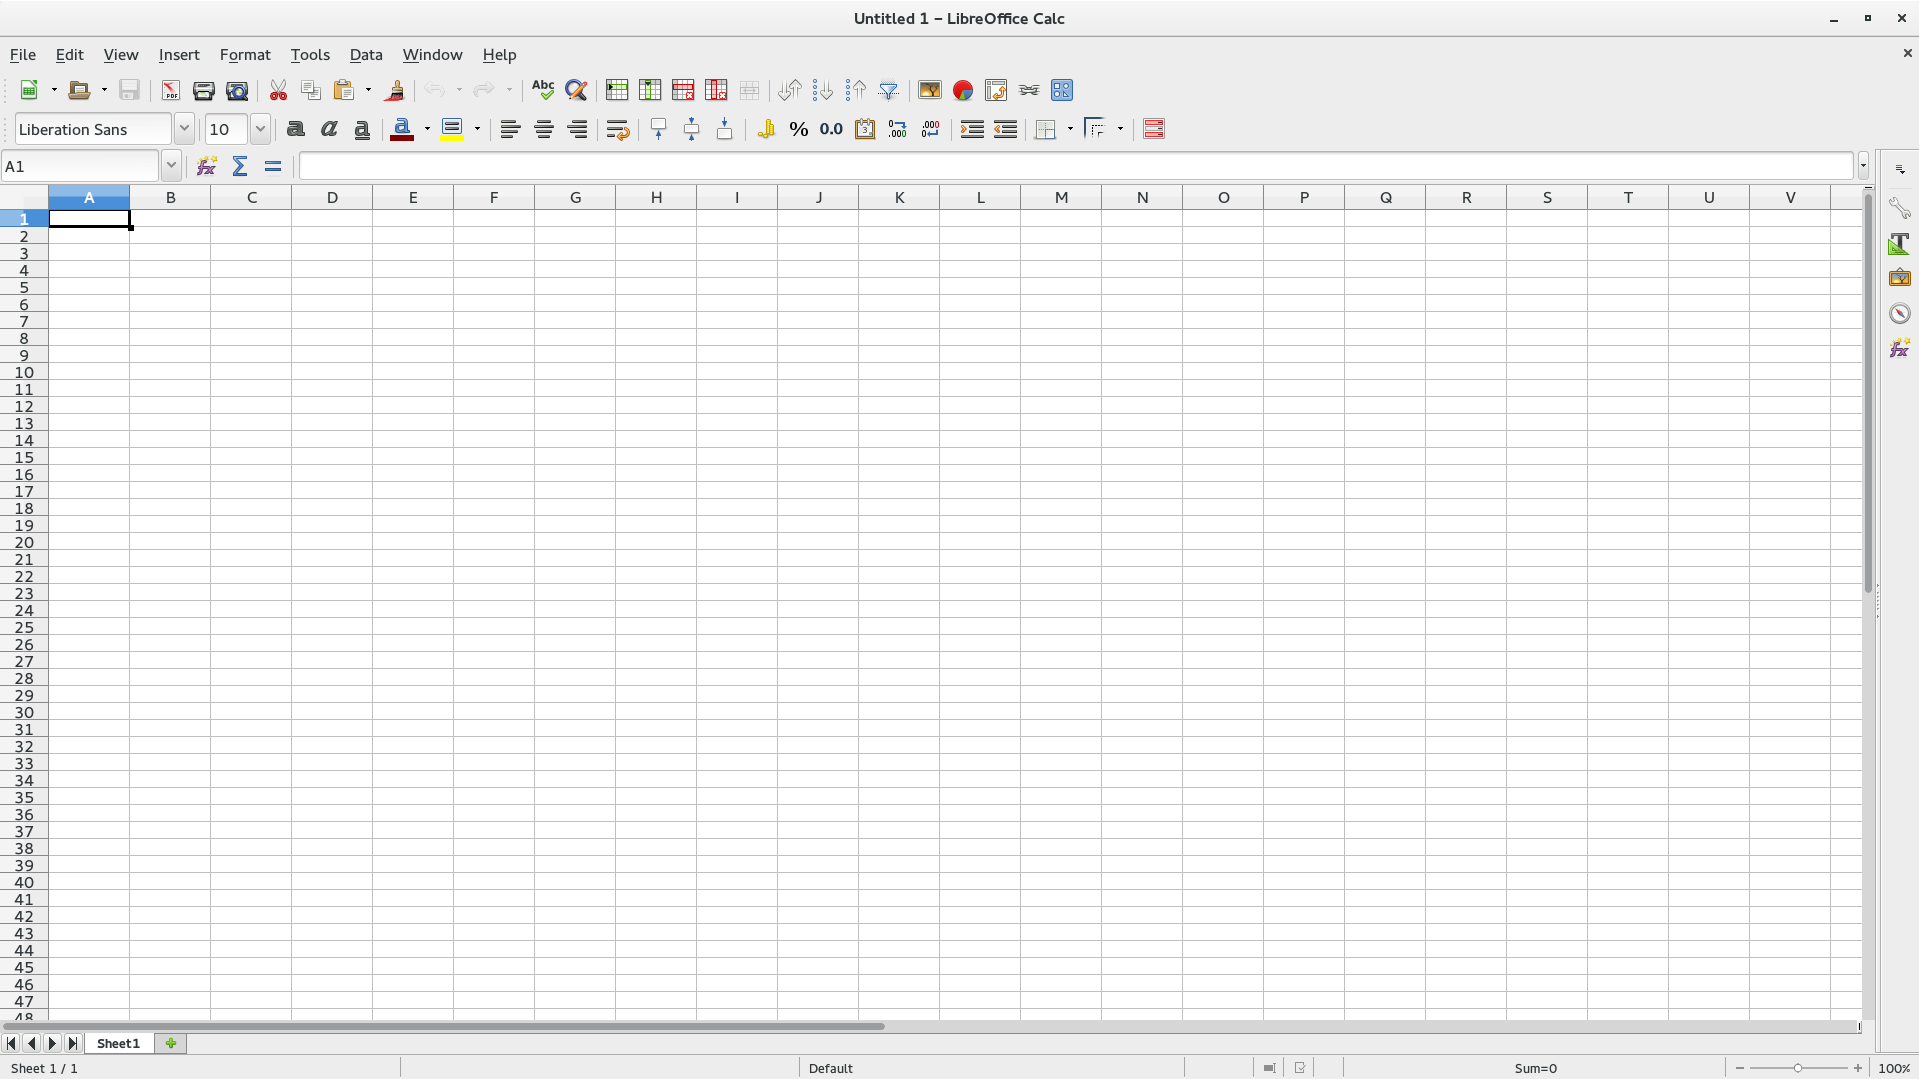
\includegraphics[width=0.8\textwidth]{./img/calculo.png}
	    \caption{Folla de cálculo}
	  \end{center}
    \end{figure}

    O sistema é moi versatil para usuarios experimentados pero implica un gran 
traballo manual e pode chegar a ser un suplicio para usuarios con poucos coñecementos de 
ofimática.

  As actas seguen a chegar en papel a federación e os datos deben ser introducidos nas 
diversas follas de cálculo (que en competicións de gran tamaño, vólvense inmanexables), 
revisando as sancións de xeito manual, polo que os erros na interpretación dos datos son 
habituáis.

\clearpage

    \subsection{Novanet}
    \santiagosays{Eu fusionaría todos estes competidores dentro dun mesmo paraguas, de
      aplicacións web xa existentes, e dentro desa sección enumeralas e contar pros e
      contras de cada unha; ou incluso distinguir simplemente entre ``old-schoool''
      (federatio/novanet) (aínda que novanet está mellorando a interface, parece) e cousas
      novas tipo miLeyenda. Eu creo que non hai moita diferencia entre cada unha delas en
      particular, pero que si que forman conxuntos distintos de funcionalidades que é
      interesante distinguir no state of the art}

    \ProTip{Podes utilizar subfigures para agrupar as capturas de algunhas das aplicacións
      web para empregar menos espacio vertical e maximizar o ancho que ocupan as túas
      figuras sen que sexan moi grandes no papel.}

      Novanet é unha empresa especializada na xestión de competicións de fútbol 
e o seu producto componse únicamente dunha aplicación web dende a que crear as 
clasificacións pero tamén modificar as actas dos partidos ou ver os resultados.

      No caso que nos incumbe, non dispón dunha aplicación que poida ser instalable nun 
teléfono móbil e os árbitros vense na obriga de acceder directamente a páxina web da 
federación para modificar as actas.
  
      Ademáis, non permite o funcionamento do sistema de forma offline xa que non foi 
pensado inicialmente para o caso, o que obriga a levar a acta en papel que se cubre 
igualmente a pesar de que logo o árbitro sube os datos a web cando chega a súa casa.

      A interfaz é bastante complexa, o cal é un problema xa que a meirande parte dos 
árbitros son de avanzada idade e polo tanto resúltalles dificil adaptarse.

      Por último mencionar que únicamente está pensada para funcionar en fútbol e fútbol 
sala.
	
      \begin{figure}[h!]
	\begin{center}
	  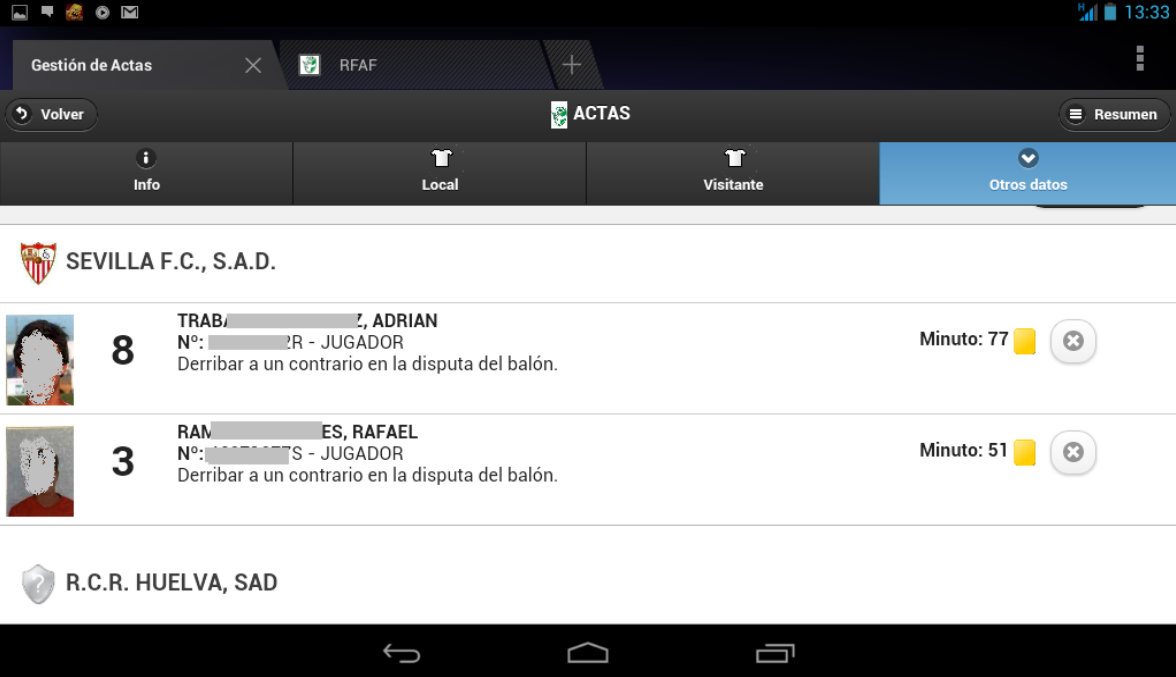
\includegraphics[width=0.8\textwidth]{./img/novanet-app.png}
	  \caption{Aplicación web de Novanet}
	\end{center}
      \end{figure}

\clearpage

    \subsection{Federatio}

    O caso de Federatio é moi similiar ao anterior xa que tampouco dispón dunha 
aplicación específica para a xestión de actas electrónicas de forma sinxela e polo tanto, 
os árbitros deben acceder a través da páxina web ao chegar a casa, para pasar os datos da 
acta física a versión electrónica.

    A interfaz dista de ser atractiva xa que apenas se renovou dende que comezou a 
funcionar entorno ao ano 2005 e non se atopa adaptada a móbiles, o que dificulta 
enormemente a labor dos árbitros.


      \begin{figure}[h!]
	\begin{center}
	  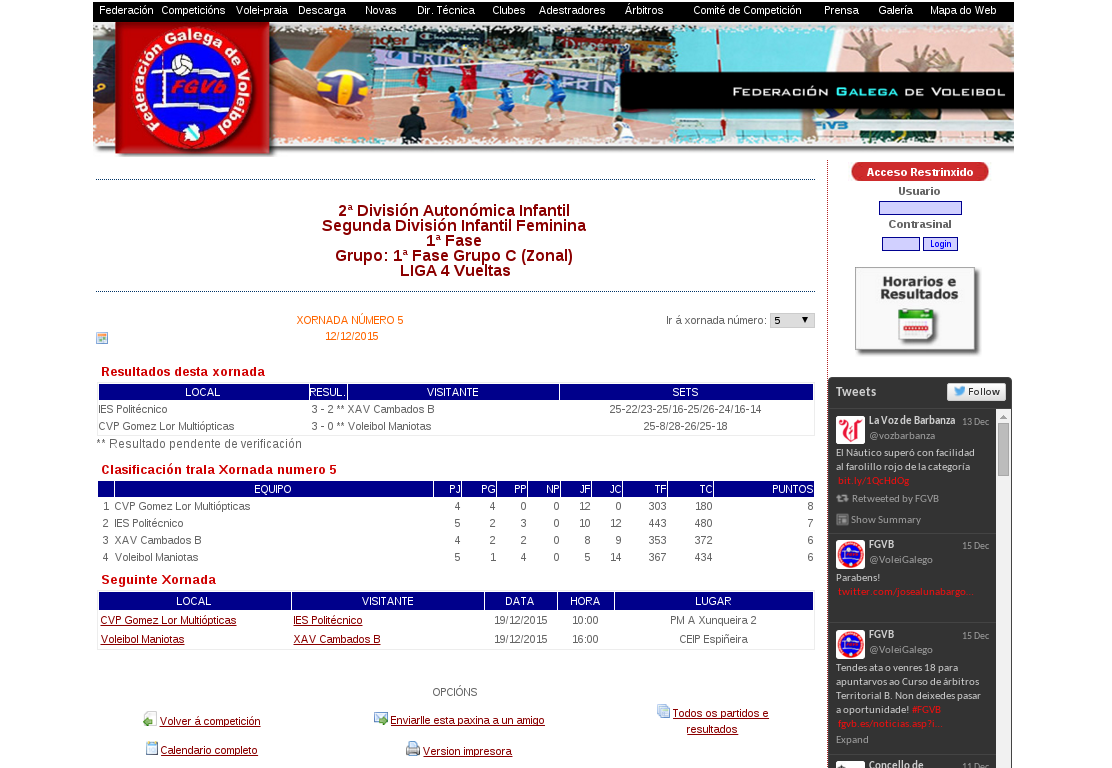
\includegraphics[width=0.8\textwidth]{./img/federatio-app.png}
	  \caption{Web da FGVB co sistema Federatio}
	\end{center}
      \end{figure}

\clearpage

    \subsection{miLeyenda}
  
    miLeyenda é unha plataforma de xestión de competicións na nube que permite 
aos administradores de federacións dispor tamén de unha aplicación móbil nativa 
para IOS e outra para Android.
    
    Dende esta aplicación poden xestionar gran parte dos parámetros das súas competicións 
entre os que se atopan as actas dos encontros.
  
    Así mesmo tamén dispoñen dunha aplicación para que os xogadores e clubes poidan ver 
os resultados e as clasificacións polo que o custe de mantemento das aplicacións elévase 
enormemente ao ter que soportar ata 4 apps móbiles diferentes.
    
    Esta é unha das grandes vantaxes de utilizar as tecnoloxías web que emprega VACmatch 
Mobile, permitíndo utilizar unha soá aplicación para calquera sistema operativo.

    A usabilidade das aplicacións é salientable e permite a xestión de diversos deportes 
pero a cambio non permite cubrir as actas de forma offline, un problema habitual ante a 
falta de cobertura nos diversos pavillóns e campos deportivos.
  
      \begin{figure}[h!]
	\begin{center}
	  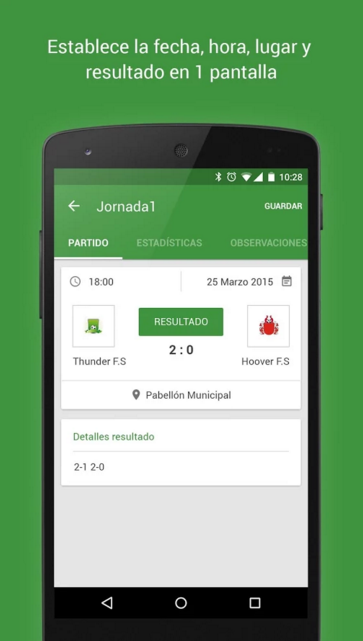
\includegraphics[width=0.3\textwidth]{./img/mileyenda-app.png}
	  \caption{APP móvil de MiLeyenda}
	\end{center}
      \end{figure}

\clearpage

    \subsection{Esportics}

    Esportics é unha startup%
    \santiagosays[]{Pero o competidor é a startup ou o software? ;-)}%
    española centrada na xestión de competicións deportivas e enfocada tremendamente cara
    o tenis e o paddel así como os deportes electrónicos.

A pesar de que a aplicación funciona para diversos deportes, a súa adaptación é bastante 
forzada en certos menús e a hora de estructurar as competicións.

    Únicamente dispón dunha páxina web adaptable a móbiles, aínda que a adaptación é 
mellorable, e polo tanto, non dispón dunha aplicación específica para que os árbitros 
poidan cubrir as actas de forma sinxela dende o seu teléfono.

    A usabilidade é aceptable pero mellorable, engadindo unha complexidade en certos 
menús que non son precisos e que provoca que os árbitros de avanzada idade, lles resulte 
tamén pouco intuitivo.

    \begin{figure}[h!]
      \begin{center}
	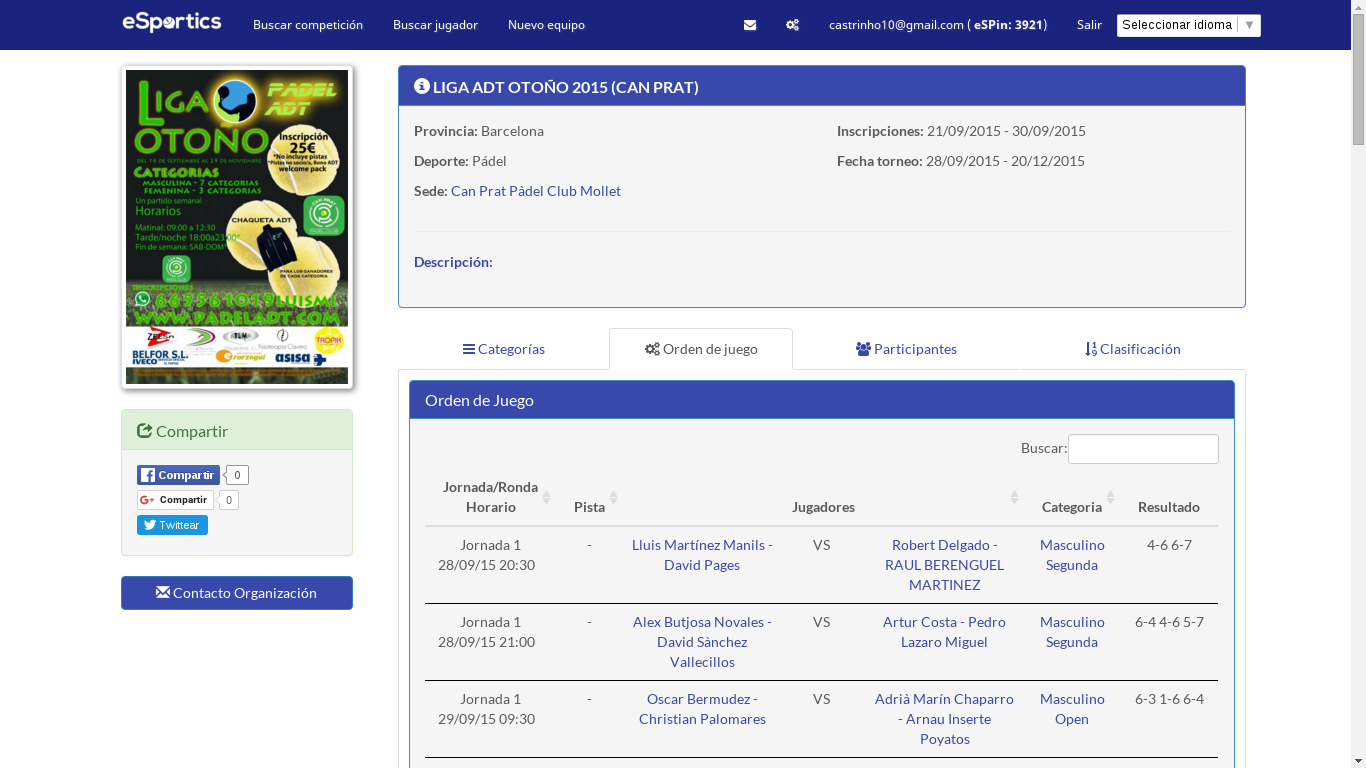
\includegraphics[width=\textwidth]{./img/esportics-app.png}
	\caption{Torneo de tenis na web de Esportics}
      \end{center}
    \end{figure}

\clearpage

    \subsection{Sportngin}

    \todo{citar desde o texto as figuras} \santiagosays{Presta
      atención á capitalización. Estou voando e non sei cal é, pero
      creo recordar que tiña outra letra maiúscula polo medio. Está ben poñerlla. Igual era a \textbf{n}?}
      
    Sportngin é unha solución integral para a xestión deportiva, probablemente un dos 
proxectos de referencia xa que dispón de aplicacións web e móbil para a xestión e a 
visualización de competicións.

    De feito, Sportngin permite a personalización da aplicación móbil a cada federación, 
cos seus logotipos, colores corporativos e incluso certos menús personalizables 
e incluso permite traballar de forma offline.
    
    A parte das funcións habituáis para xestionar as competicións e a creación de actas, 
con unha usabilidade moi coidada, aporta como valor engadido a visualización e xestión de 
noticias, fotos ou estadísticas da competición.

    Por último tamén permite aos entrenadores planificar adestramentos e incluso 
comunicarse cos seus xogadores a través da mensaxería interna.

    É sen dúbida o proxecto máis completo e a referencia a seguir.
 
    \begin{figure}[h!]
      \begin{center}
	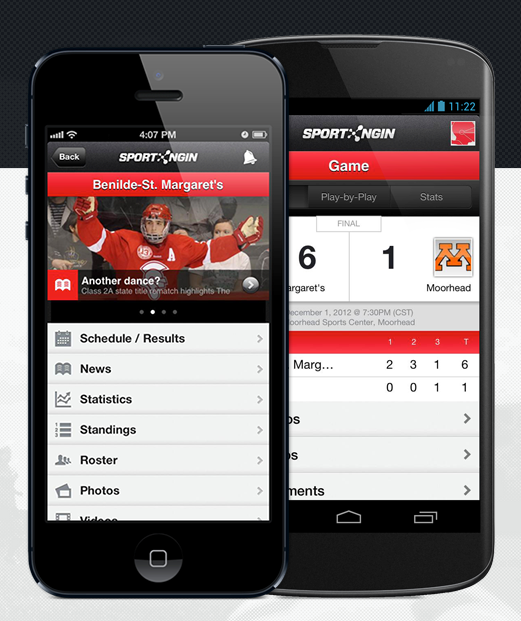
\includegraphics[width=0.5\textwidth]{./img/sportngin-app.png}
	\caption{APP móvil de Sportngin}
      \end{center}
    \end{figure}

\clearpage

    \subsection{Outras plataformas}
    Existen moitas ferramentas para a xestión de competicións e resultados pero apenas 
ningunha facilita aos árbitros unha plataforma sinxela e con unha usabilidade 
medianamente coidada.
    
    Tamén existen pequenas extensións coa idea de extender outras plataformas xenéricas 
para adaptalas a xestión de competicións como o \emph{Joomla! CMS sport extension} pero a 
función final é tremendamente limitada.
  
    Tamén temos outras propostas como \emph{Siguetuliga} que permite as persoas que 
se atopan vendo o partido, subir os resultados pero simplemente é un complemento, non 
facilita nin elimina o traballo dos xestores de competicións.

  \section{Aplicacións libres no mercado}
  
  O software libre é un sector en alza na actualidade%
  \santiagosays[]{Que significa isto? Eu esta frase só a oigo nos telexornais e nunca a
    entendín XD}, %
  os proxectos colaborativos que forman o mundo \emph{Open Source} estanse a impor en
  múltiples mercados fronte as correspondentes alternativas privativas que adoitan a ser
  tremendamente costosas.%
  \santiagosays[]{É polo custe? Éo tamén adí noutros mercados? Hai outros factores?}

    Mesmo as grandes compañías TIC están a apostar por liberar parcial ou totalmente as 
súas tecnoloxías e productos, favorecendo un desenvolvemento colaborativo fronte a idea 
atrasada de secretismo e individualismo do modelo productivo habitual.%

\santiagosays{Eu non estou dacordo con esta frase, pero non sei se é porque opinamos
  distinto ou porque non a esté entendendo. A miña opinión é que as grandes (Google,
  Apple) liberan o código do que non é relevante dende o punto de vista diferenciador,
  pero non comparto a idea de que o secretismo sexa cousa atrasada e do pasado: non vexo
  a Google liberando o algoritmo do seu motor de busca, nin a Netflix, Apple ou Google
  liberando os seus respectivos datasets de recomendacións, Siri ou \emph{calquera
    cousa}, respectivamente. Google liberou o toolkit de Deep Learning (pero non os
  datos cos que o usan) porque precisamente se outros lles axudan coa base, seguirán
  sendo os mellores no mercado, porque teñen os mellores segredos igualmente.}

Concretamente no mundo do deporte é tremendamente complicado atopar algún exemplo de
aplicación baseada en software libre e as poucas existentes como \emph{zuluru} ou
\emph{phpmysport} atópanse tremendamente atrasadas, tanto en funcionalidades como no
aspecto visual e por suposto sen ningún tipo de aplicación móbil para facilitar a
xestión das actas polo que é importante propor unha alternativa ás aplicacións
privativas habituais como é VACmatch Mobile.

\santiagosays{Tremendamente atrasadas é unha expresión que usas ao longo da memoria
  bastante, e non é moi formal que digamos. Ademais de que é un xuízo de valor: un texto
  expositivo desta natureza debería de enfocarse en feitos contrastables todo o posible} %

  \section{Solución aberta e adaptable}
  \santiagosays{Céntraste moito na gratuidade da cousa, cando o interseante do software
    libre é máis a capacidade de personalización: a alguén vas a ter que pagarlle igual
    para que o faga, pero se xa hai algo de base, pois tes máis independencia respecto a
    a quen lle pagas e podes aproveitar o innovado polos demais.}%

  Os xestores de competicións habitualmente realizan unha considerable inversión 
económica para que unha empresa de consultoría lles cree unha aplicación web ou de 
escritorio a medida para a súa xestión. Algunhas mesmo dispoñen de aplicacións móbiles 
para os árbitros pero que son específicas para dito sistema de xestión polo que a 
reutilización de aplicacións non é posible.

  Ademáis, estos sistemas son propietarios e o código non se atopa accesible 
polo que é imposible tratar de adaptar ditas aplicacións móbiles para outros 
sistemas de xestión.

  É por isto polo que se chegou a conclusión de que é preciso crear unha 
plataforma aberta como é VACmatch Mobile que porporciona unha aplicación 
software libre adaptable a diversos deportes e integra unha API de comunicacións 
aberta para a xestión de actas electrónicas e que permita a súa integración 
noutros sistemas de xestión entre os cales se atopa o sistema de VACmatch, unha 
implementación libre para a xestión de competicións.

  
%%% Local Variables:
%%% mode: latex
%%% TeX-master: "../root"
%%% End:

\chapter{Metodoloxía}
\minitoc
% \label{chap:Metodoloxia}
% \vspace{0.5cm}

%%%%%%%%%%%%%%%%%%%%%%%%%%%%%%%%%%%%%%%%%%%%%%%%%%%%%%%%%%%%%%%%%%%%%%%%%%%%%%%%
% Objetivo:                        %
%%%%%%%%%%%%%%%%%%%%%%%%%%%%%%%%%%%%%%%%%%%%%%%%%%%%%%%%%%%%%%%%%%%%%%%%%%%%%%%%

  \lettrine{N}{este} capítulo imos analizar as diversas metodoloxías utilizadas para a 
xestión do proxecto e explicar a adaptación das mesmas que finalmente se utilizóu.

  Comezaremos falando da metodoloxía orientada ao modelo de negocio xa que, 
como se indica na introdución, este proxecto xurdíu dentro de unha iniciativa 
empresarial e polo tanto dende o primeiro momento se traballou orientado cara o 
cliente, convertíndoo nun dos pilares do desenvolvemento.

  Seguidamente comentaremos as metodoloxías áxiles que serviron de base para 
definir a metodoloxía utilizada finalmente, unha adaptación das mencionadas e 
que tamén se indica para rematar o capítulo.

  \section{Lean Startup}
  Lean Startup\cite{book:leanstartup} é unha metodoloxía para abordar o 
lanzamento de negocios e produtos a través da validación, a experimentación e a 
iteración no lanzamento dos mesmos co fin de acortar o ciclo de desenvolvemento.

  É unha metodoloxía de traballo moi habitual nas startups que se centra na 
idea de \emph{Crear - Medir - Aprender}, desenvolvendo pequenos produtos e 
realizando tests de mercado reais con verdadeiros clientes co fin de medir o 
seu grao de satisfación e aprender para mellorar o produto en seguintes 
iteracións.

  Habitualmente céntrase na idea de crear un MVP (Minimum Viable Product), 
unha versión do producto que permite os desenvolvedores recoller co mínimo 
esforzo a máxima cantidade de coñecemento validado por parte dos clientes, 
evaluando as hipóteses de se os clientes realmente estarían dispostos a pagar 
polo producto e implicando a dito cliente no desenvolvemento do produto.

  \section{eXtreme Programming}
  eXtreme Programming\cite{book:agile} é unha metodoloxia de desenvolvemento 
áxil e incremental baseada na integración do cliente no desenvolvemento así como 
na simplicidade do código.

  A metodoloxia aposta por facer as cousas sinxelas, sen preocuparse por ter 
que facer un pequeno traballo por adaptalas se é preciso, fronte a idea 
tradicional de facer un gran traballo para quizáis nunca chegar a utilizar 
parte do mesmo.

  As entregas funcionais son frecuentes e outras características como a 
importancia de introducir a programación en parellas para reducir o número de 
erros que se producen ao programar.

  Por último aboga por introducir o TDD (Test Driven 
Development)\cite{book:cleancode}, implementando primeiro os tests, 
verificando que fallan, para a continuación implementar o código que fai que 
pasen correctamente os mesmos.
  A idea é que os requisitos sexan convertidos a probas e de este modo cando os 
tests se pasen, poderemos garantizar que o código cumple os requisitos.

  \section{Scrum}
  Scrum\cite{book:scrum} tamén é unha metodoloxía incremental de desenvolvemento 
cunha serie de roles definidos para o proceso, cada un coas súas 
responsabilidades e que divide o proxecto en varios \emph{Sprints} que son 
ciclos de desenvolvemento.

  Cada un de eles ten unha duración definida polo equipo de, habitualmente, 
entre unha e catro semanas, proporcionando un incremento de software entregable 
ao final de cada \emph{Sprint}.

  A totalidade das tarefas do proxecto atópanse definidas e priorizadas en unha 
lista chamada \emph{Product Backlog}. Para cada sprint, selecciónanse aquelas 
tarefas que determinarán a lista a implementar durante a presente iteración, o
\emph{Sprint Backlog}, e que non pode variar ata rematar o sprint.

  Durante todo o ciclo de traballo realízanse reunións diarias para comprobar o 
estado do proxecto así como outras ao finalizar e ao comezar os sprints, co 
fin de analizar a iteración anterior e planificar a seguinte, facendo un 
seguimento continuo do proxecto e facilitando a adaptación do mesmo a posibles 
novos requisitos.

  \section{Adaptación da metodoloxía}

    \subsection{Desenvolvemento orientado ao cliente}
      O proxecto ten lugar dentro dunha iniciativa empresarial polo que se 
decidíu utilizar un modelo de desenvolvemento orientado ao cliente en todo 
momento, baseandose no pilar central da metodoloxia \emph{Lean Startup}.

    Para isto realizáronse diversas visitas as federacións para comprobar as 
súas necesidades a través dunha serie de entrevistas estructuradas para 
coñecer os problemas e a súa prioridade a hora de resolvelos.

    Do mesmo modo realizáronse dous prototipos, un primeiro únicamente 
con plantillas HTML para testear a organización da interfaz de usuario e un 
segundo xa funcional para comprobar a resposta dos usuarios finais ante o seu 
funcionamento.

    \subsection{Sprints con backlog adaptable}
    A organización do desenvolvemento organizouse de xeito moi similar a idea 
proposta en \emph{Scrum}, dividindo o proceso en sprints, pequenas iteracións 
de dúas ou tres semanas de duración e que cada unha proporciona unha serie de 
novas funcións.

    Cada sprint comeza con unha reunión de aproximadamente 30/45 minutos de 
duración na que realizar a planificación do mesmo en función do 
traballo realizado no sprint anterior, o que permite realizar melloras nas 
previsións segundo o aprendido dos anteriores.

    A diferencia do proposto por Scrum, decidíuse optar por sprints de duración 
variable e con un backlog adaptable según as necesidades xa que proporciona 
unha maior flexibilidade e liberdade.

    \subsection{Reunións semanais}
    Todas as semanas faise unha reunión de 30/45 minutos de duración na que 
analizar o realizado na semana anterior e comprobar o seguimento da iteración 
co fin de atopar desviacións e corrixilas.

    Cando unha reunión semanal coincide co fin de un sprint, dita reunión 
sirve para realizar a planificación do seguinte sprint de xeito moi similiar as 
reunións de sprint que se realizan en \emph{Scrum}.

    \subsection{Reunións diarias}
    Ao comezar o día realízase unha análise duns 10 minutos de duración para 
revisar o realizado no día anterior e planificar de forma máis concreta o que 
se vai facer ese mesmo día.

    \subsection{Releases}
    Durante o desenvolvemento do proxecto trátase de aplicar a idea de realizar 
unha serie de pequenos entregables en cada iteración.

    Todas as entregas ao finalizar unha iteración son totalmente funcionais 
pero non todas son versións entregables reais para ser postas en produción.

    Durante o desenvolvemento producíronse 3 entregas (\emph{releases}) 
totalmente funcionais, a primeira foi un prototipo, a segunda foi a versión 
real do proxecto e a terceira incorporou tests e diversas características para 
asegurar unha primeira versión estable.

    \subsection{Simplicidade}
    Utilizouse o principio de simplicidade que promove \emph{eXtreme 
Programming}durante todo o desenvolvemento baixo a máxima de implementar 
únicamente o imprescindible en cada momento, sempre pensando en programar 
para hoxe e non para mañá.

    A idea fundaméntase en realizar refactorizacións de código para engadir 
novas funcionalidades a medida que son necesarias en lugar de invertir 
demasiado tempo na planificación e implementación de funcións que se supoñen 
necesarias e, algunhas das cales, é probable que non sexan utilizadas
finalmente.

    \subsection{Tests}
    A importancia de creación de tests automatizados está totalmente 
demostrada, atopándose en auxe metodoloxías como
TDD~(Test~Driven~Development)%
\footnote{Desenvolvemento dirixido polos tests.} %
ou BDD~(Behaviour~Driven~Development)%
\footnote{Desenvolvemento dirixido polo comportamento} %
que tratan de dirixir o desenvolvemento a través dos tests e
que son realizados antes da implementación da funcionalidade.

    Durante a primeira parte do desenvolvemento non se aplicou ningunha de 
estas metodoloxías pero a partir da primeira \emph{release} e da integración 
dos primeiros tests, decidíuse optar por aplicar TDD no desenvolvemento, 
realizando probas unitarias nos servicios utilizados.

    \subsection{Fluxo de contibución ao proxecto}
    O fluxo de traballo utilizado dende o primeiro día trata de simular o 
traballo diario de equipo e permite controlar a evolución do código de xeito 
máis ordenado.

    Disponse de unha rama \emph{master} na que se atopa a versión estable de 
desenvolvemento así como de unha rama \emph{development} que é máis inestable e 
que ao final de cada sprint, é integrada dentro de \emph{master}.

    Unha nova funcionalidade ou erro é resolto nunha nova rama independente,
creada a partir de \emph{development} e tratando que todas estas novas 
funcionalidades sexan independentes entre si.

    Así mesmo tratase de que todos os \emph{commits} sexan funcionais e o máis 
independentes posibles, evitando ter algún que non compile ou que non pase 
os tests.

    Posteriormente realizase unha \emph{pull request}\footnote{Unha pull 
request é unha petición para integrar unha rama de Git en outra a través de 
GitHub, un mecanismo habitual para engadir novas funcionalidades ou correxir 
erros.} a través do mecanismo que proporciona o repositorio 
de código de GitHub, esperando que alguén revise o código para ser 
integrado na rama de desenvolvemento.

    Cada certo tempo revísanse as \emph{rull requests} abertas, analízase o 
codigo e se todo é correcto, acéptase.

    Ao final de cada sprint realízase una nova \emph{rull request} para 
integrar a funcionalidade creada no sprint actual e que se atopa na rama de 
desenvolvemento, dentro da rama estable.

    Dende a introducción de tests no proxecto, todo código subido ao 
repositorio é analizado a través dun sistema de integración continua
---que se comenta con máis detalle na Sección~\ref{sec:travis},--- e que comproba se os cambios 
engadidos pasan os tests ou non, e avisan por correo 
electrónico do resultado.


%%% Local Variables:
%%% mode: latex
%%% TeX-master: "../root"
%%% End:

\chapter{Análise de requisitos globais}
\minitoc
% \label{chap:Analisederequisitosglobais}
% \vspace{0.5cm}

%%%%%%%%%%%%%%%%%%%%%%%%%%%%%%%%%%%%%%%%%%%%%%%%%%%%%%%%%%%%%%%%%%%%%%%%%%%%%%%%
% Objetivo:                        %
%%%%%%%%%%%%%%%%%%%%%%%%%%%%%%%%%%%%%%%%%%%%%%%%%%%%%%%%%%%%%%%%%%%%%%%%%%%%%%%%

  \lettrine{N}{este} capítulo exporemos o proceso de análise de requisitos 
para o desenvolvemento do proxecto, explicando as diversas visitas que se 
realizaron a múltiples federacións.

  Durante meses traballouse da man de varias de estas federacións e asociacións 
deportivas tratando de comprender, non só as necesidades reais dos clientes se 
non tamén traballando na usabilidade da aplicación da súa man.

  Comezaremos vendo as suxerencias recibidas das diversas federacións e 
finalmente expoñeremos os requisitos que finalmente se decidíu engadir ao 
proxecto.

  \section{Consultas a xestores de federacións}
  Para a realización deste apartado decidiuse consultar con diversas 
asociacións deportivas e federacións das que obter suxerencias e peticións 
acerca das necesidades que actualmente están a demandar, co fin de obter certas 
funcionalidades a implementar e incluso a priorización segundo as súas
necesidades máis urxentes.

Na realización deste apartado contouse coa colaboración das asociacións e 
federacións deportivas que se detallan a continuación.

  Tras varias reunións con eles, obtívose unha lista de requerimentos e 
suxerencias respecto das súas necesidades, que están detalladas 
na Sección~\ref{sec:analisis:obtido}, e dos que finalmente foron destilados os 
requisitos finais, que son presentados como 
Sección~\ref{sec:analisis:requisitos} de este capítulo.

  \begin{description}

  \item [Asociación de peñas de fútbol de A Coruña].
  É a asociación máis interesada polo proxecto e coa que se leva colaborando 
dende o primeiro momento, aportando suxerencias e incluso novos colaboradores 
para poder desenvolver un producto de calidade.

  Realizáronse ata 5 visitas á federación co fin de mostrarlles a evolución do 
proxecto, comprobar a usabilidade da aplicación e o estado das funcionalidades.

  \item [UPOFU].
  A Asociación de peñas ten boa relación coa UPOFU polo que nos facilitóu o seu 
contacto e ofrecéronse da mesma maneira a colaborar co proxecto, interesados 
tamén en incorporalo na súa xestión.

  \item [Torneo VACmatch].
  Organizóuse un torneo de fútbol sala co fin de testear o primeiro prototipo 
do proxecto con usuarios reais, tanto árbitros como xogadores e no que se 
comprobou as dificultades dos usuarios e se verificou a súa necesidade de 
dispor deste tipo de ferramentas.

  \item [Outras].
  Tamén se realizaron visitas a outras federacións incluso de outros deportes 
como o voleibol para comprobar os seus problemas na xestión e verificar a 
importancia de que o proxecto sexa facilmente adaptable a outros deportes.

  \end{description}

  \section{Peticións obtidas}
  \label{sec:analisis:obtido}
    \begin{description}
     \item [Cubrir acta en tempo real]. A aplicación móbil debe permitir cubrir 
as actas e actualizar os resultados en tempo real co fin de manter a web da 
federación actualizada en todo momento.

     \item [Permisos]. Débese dispor dun sistema de permisos para diferenciar a 
árbitros e outros xestores da competición.

     \item [Sincronización]. A aplicación móbil debe sincronizar os datos coa 
plataforma central onde se atopa o sistema de xestión da federación e a súa web.

     \item [Persoas convocadas]. É preciso poder dispor de todas as persoas 
inscritas nun equipo e poder indicar de xeito sinxelo si esas persoas están ou 
non no encontro.

     \item [Eventos]. A aplicación debe poder crear novos eventos, borralos e 
mostralos de xeito sinxelo e ao mesmo tempo de xeito xenérico que permita 
integrar calquera deporte.

     \item [Motivación dun evento]. Debe poderse incluir en certos eventos un 
motivo polo que se creou ese evento, dispoñendo dunha lista de motivos por 
defecto e incluso permitindo ao xestor da federación, engadir novos motivos 
personalizados para a súa federación.

     \item [Editar dorsal dun xogador]. Xa que en moitas competicións un 
xogador pode xogar cada partido con un dorsal diferente, debe poder cambiarse o 
dorsal por defecto dende a aplicación móbil.

     \item [Persoa con varios roles]. Debe terse en conta a posibilidade de que 
unha persoa poida ter varios roles, tanto de xogador como de entrenador dentro 
de un equipo.

    \end{description}

  \section{Requisitos finais}
  \label{sec:analisis:requisitos}
  \subsection{Usuarios}

    \begin{itemize}

    \item \textbf{Facer login e logout}.
    A aplicación móbil debe permitir iniciar e pechar sesión para os árbitros.

    \item \textbf{Permisos para edición de actas}.
    A aplicación de xestión disporá de permisos diferenciados para editar as 
actas xa que os árbitros únicamente poden editar as actas que teñen asignadas.

    \end{itemize}

  \subsection{Listar actas}

    \begin{itemize}

    \item \textbf{Visualizar próximas actas a cubrir dun árbitro}.
    Mostrar a lista de próximas actas que ten para cubrir un árbitro, mostrando 
o lugar e a data do mesmo para facilitar o seu traballo.

    \item \textbf{Visualizar actas cubertas dun árbitro}.
    Debe mostrar as actas cubertas anteriormente e todos os seus datos.

    \item \textbf{Actualización automática de actas descargadas ante 
modificacións}.
    As actas deben actualizarse de forma automática na aplicación do árbitro 
unha vez o xestor da federación realiza a asignación dun partido a un colexiado.

    \end{itemize}

  \subsection{Visualizar actas}

    \begin{itemize}

    \item \textbf{Listar o personal e xogadores dun equipo}.
    Móstrase o personal e os xogadores do equipo na aplicación móbil.

    \item \textbf{Visualizar datos xerais dun acta}.
    Débese mostrar do xeito máis simplificado posible os datos xerais da acta 
nunha pantalla inicial para facilitar que sexa cuberta interactivamente durante 
o desenvolvemento do encontro.

    \item \textbf{Visualizar eventos dun acta}.
    Permitirase visualizar os eventos ordenados cronolóxicamente para facilitar 
a súa consulta.

    \end{itemize}

  \subsection{Xeración de actas offline}
  A aplicación debe permitir a creación de actas de forma offline xa que pódese 
dar o caso de que a aplicación móbil non actualice as novas actas e o árbitro 
se vexa na obriga de crear unha acta de forma manual.

  \subsection{Modificación de actas}

    \begin{itemize}

    \item \textbf{Modificación de propiedades da acta}.
    Débese permitir modificar propiedades da acta tales como a localización 
do encontro ou a data do mesmo.

    \item \textbf{Convocar un xogador ou entrenador}.
    A aplicación móbil permitirá indicar qué personal dos equipos están 
presentes no encontro así como editar certos datos dos mesmos como o seu dorsal.

    \item \textbf{Engadir un xogador que non está no equipo}.
    Pode darse o caso de que a un xogador débeselle permitir xogar un encontro 
aínda que non fose dado de alta na federación correspondente polo que é preciso 
poder engadir novos xogadores.

    \item \textbf{Editar datos de persoal creado}.
    Débese permitir editar certos datos dun xogador que foi creado dende 
a aplicación móbil como o nome, o dorsal ou o equipo o que pertencen.

    \item \textbf{Poder engadir motivos dun evento xerado}.
    A federación debe poder engadir novos motivos personalizados para poder 
engadir a un evento dende a aplicación de xestión.

    \item \textbf{Cambiar de parte}.
    A aplicación móbil debe permitir cambiar de parte no encontro.

    \item \textbf{Modificar o tempo}.
    A aplicación móbil disporá dun cronómetro que permita seguir o tempo do 
encontro así como permitirá modificalo manualmente por si hai algún desaxuste 
durante o encontro.

    \item \textbf{Engadir observacións na acta}.
    O árbitro debe poder engadir observacións as actas dos encontros.

    \item \textbf{Asinar a acta}.
    Tanto persoal do equipo como árbitros deben poder asinar as actas con un 
código PIN do que disporá cada un.

    \item \textbf{Engadir eventos deportivos}.
    A aplicación debe facilitar a adaptación de novos deportes e a posibilidade 
de engadir de xeito sinxelo novos eventos.

    \end{itemize}


\chapter{Planificación e seguimento}
\minitoc
% \label{chap:Planificacioneseguimento}
% \vspace{0.5cm}

%%%%%%%%%%%%%%%%%%%%%%%%%%%%%%%%%%%%%%%%%%%%%%%%%%%%%%%%%%%%%%%%%%%%%%%%%%%%%%%%
% Objetivo:                        %
%%%%%%%%%%%%%%%%%%%%%%%%%%%%%%%%%%%%%%%%%%%%%%%%%%%%%%%%%%%%%%%%%%%%%%%%%%%%%%%%

  \lettrine{E}{n} este capítulo...

  \section{VACmatch validación de negocio. Agosto 2015 - Outubro 2015}
  blabla empresa, clientes, GOF y Yuzz, torneo de testing

    \subsection{MVP}
    Validación de usuario con tests de laboratorio sobre versión sin funcionalidade
    1 mes

    \subsection{MVP funcional}
    Creación de APP sinxela para tests de campo reais.
    2 mes
      \paragraph{Planificación temporal}
      \paragraph{Definición da iteración}
      \paragraph{Feedback}
      \paragraph{Tarefas e seguimento}

  \section{VACmatch desenvolvemento de produto. Outubro 2015 - Xaneiro 2016}
  Ronda de inversión, incrición cusl, blog vacmach

    \subsection{1ª iteración. Creación do proxecto}
    Aprender PouchDB, deseño da estructura e arquitectura, deseño modelo de datos, listar 
  actas.

    \subsection{2ª iteración. Xestión de actas}
    Ver o resumo dun acta xenérica, cronómetro e control do tempo 

    \subsection{3ª iteración. Eventos}
    Xestión de eventos xenérica, sport events e control events, actualizar resultados na 
  acta, listar e borrar eventos, convocar xogadores,, listar eventos

    \subsection{4ª iteración. Xestión de usuarios e creación offline de actas}
    login, logout, metese staff, crear actas offline
    Memoria, 3 primeros apartados

    \subsection{5ª iteración. Sinaturase}
    Sinaturas con PIN, engadir incidencias
    do sprint anterior: crear usuario, crear árbitro ao crear user

  \section{VACmatch de empresa a comunidade. Xaneiro 2016 - Maio 2016}
    \subsection{6ª e 7ª iteración. Optimización e melloras}
    Refactor de servizos creando un xenérico, crear clases para cada entidade e simplificar o código
    creación aleatoria de ids

    \subsection{8ª iteración. Testing e integración continua}
    Tests servicios, travis e confirmar contrasinal e PIN

    \subsection{9ª e 10ª iteración. Inxección de dependencias}
    Corrección de erros na CI, engadir textos de error, creación de snackbar para erros e comunicacións
    Inxección de dependencias -> motivo dependencias circulares
    Estados no report: pasar de isFinished -> Ready, Started e Finished

    \subsection{Release 0.2.0: Usabilidade en menús}
    Links en menus e engadir información e documentación en github (instalación, DB, etc)

    \subsection{Release 0.2.1: I18n e app híbrida}
    React intl, cordova, documentación instalación en Android

    \subsection{Release 0.2.2: Imáxe corporativa e revisión de erros}
    Imaxe corporativa VACmatch, bugfix
    Memoria a saco

    \subsection{Release 0.3.0: Usabilidade móbil e entrega continua}
    Por cordova: dialogos -> ventás, transición carga, migrar taiga.io, Travis + Docker
\chapter{Fundamentos tecnolóxicos}
\minitoc
% \label{chap:Fundamentostecnoloxicos}
% \vspace{0.5cm}

%%%%%%%%%%%%%%%%%%%%%%%%%%%%%%%%%%%%%%%%%%%%%%%%%%%%%%%%%%%%%%%%%%%%%%%%%%%%%%%%
% Objetivo:                        %
%%%%%%%%%%%%%%%%%%%%%%%%%%%%%%%%%%%%%%%%%%%%%%%%%%%%%%%%%%%%%%%%%%%%%%%%%%%%%%%%

  \lettrine{N}{este} capítulo móstraranse as diversas tecnoloxías que foron 
empregadas durante o desenvolvemento do proxecto así como ferramentas de 
xestión, bases de datos, repositorios de código e ferramentas documentais, 
todas, tecnoloxías Software Libre.

  \section{Linguaxes e frameworks empregados}

  \begin{description}
   \item [ReactJS] 
\href{https://facebook.github.io/react/}{facebook.github.io/react} \\ React é 
unha librería de Javascript para a 
creación de Single Page Aplications (SPAs), permitindo crear aplicacións 
completas que se executen no navegador de forma sinxela a través de diversos 
compoñentes que se agrupan e que permiten crear aplicacións multiplataforma.

   \item [Reflux] \href{https://github.com/reflux/refluxjs}{
github.com/reflux/refluxjs}\\ É unha implementación da 
arquitectura Flux que explicaremos no Capítulo~\ref{sec:design:react} e que 
permite un fluxo de datos unidireccional, en lugar do 
bidireccional que é habitual nas aplicacións web.
    Permite tamén a creación de Stores nas que se mantén o estado das aplicacións e que 
permite compartir dito estado entra os diversos compoñentes da aplicación.

   \item [Jest] 
\href{https://facebook.github.io/jest/}{facebook.github.io/jest}\\ É unha 
ferramente sinxela creada sobre o 
framework de testing para Jasvascript, Jasmine, que facilita a utilización de 
mocks e a creación de tests unitarios.

   \item [React Intl (i18n)]\href{http://formatjs.io/}{formatjs.io}\\ React 
Intl é unha 
ferramenta para facilitar a internacionalización de aplicacións Javascript e 
concretamente as 
aplicacións baseadas en React.

   \item [React 
Router]\href{https://github.com/reactjs/react-router}{
github.com/reactjs/react-router}\\ Unha 
librería para o enrutado de aplicacións baseadas en ReactJS 
proveendo unha API sinxela con funcionalidades de gran potencia como a carga preguiceira 
de código ou o enrutado dinámico.

   \item [Material UI] 
\href{http://www.material-ui.com/}{material-ui.com}\\ Un conxunto de 
compoñentes para React que implementan o Material 
Design impulsado por Google, unha nova linguaxe visual baseada na representación en 3D 
dos obxectos que non deben intersecarse se non que a través de sombras para simular 
diferentes profundidades, os obxectos debe superpoñerse uns sobre os outros.

  \end{description}

  \section{Bases de datos}

  \begin{description}

     \item [CouchDB] \href{http://couchdb.apache.org/}{couchdb.apache.org} É 
unha base de datos 
pensada para web que permite almacenar 
os datos en formato JSON e acceder aos mesmos a través dun navegador via HTTP, 
funcionando como unha API REST (Representational state 
transfer).

  Permite múltiples funcionalidades pouco habituais entre os sistemas de 
xestión de bases de datos como servir aplicacións directamente dende 
CouchDB así como un sistema de replicación incremental e de detección de 
conflictos.

     \item [PouchDB] \href{https://pouchdb.com/}{pouchdb.com}\\ Unha base de 
datos NoSQL 
baseada en Javascript e inspirada 
en CouchDB, pensada para facilitar o funcionamento de aplicacións web de forma 
offline.

PouchDB permite almacenar os datos localmente no navegador web cando non 
hay conexión a internet e sincronizar de forma sinxela ditos datos en remoto con 
CouchDB e outros servidores compatibles.%

  \end{description}

  \section{Estándares de comunicación}

  \begin{description}
   \item [JSON] \href{http://couchdb.apache.org/}{couchdb.apache.org}\\ É un 
formato estándar para o 
intercambio de datos e que pola súa 
simplicidade estase a impoñer como formato habitual por exemplo, para a comunicación con 
APIs Rest e debido a súa similitude coa definición de obxectos en Javascript, permite que 
sexa tremendamente sinxelo traballar con él dende esta linguaxe.
  \end{description}

  \section{Repositorios de código}

  \begin{description}
   \item [Gerrit] 
\href{https://www.gerritcodereview.com/}{gerritcodereview.com}\\ Gerrit é 
un repositorio de código baseado no sistema de control de 
versións Git e centrado en proveer un xeito sinxelo de realizar revisións de 
código dende unha plataforma web. Foi utilizado durante o desenvolvemento do 
prototipo da aplicación pero finalmente decidíuse trasladar o código a GitHub 
para facilitar a colaboración de outros posibles desenvolvedores.
   \item [GitHub] \href{http://github.com/}{github.com}\\ GitHub é un 
repositorio de 
código que se está a convertir no lugar máis 
importante de publicación de aplicacións Software Libre e que permite aloxar proxectos 
como o presente, de forma totalmente gratuita.
  Cómpre destacar que esta é a única ferramenta utilizada para o desenvolvemento do 
proxecto que non é software libre pero si proporciona unha visibilidade de cara a 
comunidade de gran importancia neste tipo de proxectos.
  \end{description}

  \section{Ferramentas de xestión}

  \begin{description}
   \item [Git] \href{https://git-scm.com/}{git-scm.com}\\ É un sistema de 
control de 
versións software libre con grandes funcionalidades e que é utilizado en 
millóns de proxectos. Aporta unha versatilidade enorme ao ser distribuido, 
permitindo traballar incluso de forma offline.
   \item [Gulp] \href{http://gulpjs.com/}{gulpjs.com}\\ Un sistema que permite 
a 
automatización de tarefas durante o desenvolvemento de aplicacións como por 
exemplo compilar automáticamente o código Javascript escrito na súa última 
versión á versión máis antiga para que poida ser executada por calquera 
navegador web.
    \item [Babel] \href{https://babeljs.io/}{babeljs.io}\\ É un compilador de 
Javascript que permite a traducir código fonte escrito no estándar ECMAScript 6 
a ECMAScript 2015, soportado pola gran maioría de navegadores.
    \item [Browserify] \href{http://browserify.org/}{browserify.org}\\ É unha 
ferramenta 
que permite escribir os módulos da aplicación como se fosen módulos para unha 
aplicación escrita en Node.js e que os compila para poder ser utilizados no 
navegador web.
   \item [Redmine] \href{http://www.redmine.org/}{redmine.org}\\ É unha 
ferramenta de 
xestión de proxectos flexible, multiplataforma e software libre con diversos 
plugins para facilitar a planificación de iteracións e traballar con 
metodoloxías áxiles de desenvolvemento.
   \item [Travis CI] \href{https://travis-ci.org/}{travis-ci.org}\\ É unha 
ferramenta de 
integración continua que permite automatizar a execución de tests ou o 
despregamento automático de código. Ademáis dispón dunha integración con Github 
polo que resulta moi sinxelo automatizar estas tarefas.
   \item [Docker] \href{https://www.docker.com/}{docker.com}\\ É un sistema 
que permite 
empaquetar e despregar de xeito sinxelo aplicacións coas súas dependencias en 
unidades estándar chamadas contenedores, abstraendo e automatizando a 
virtualización da plataforma na que correrá a aplicación.
   \item [Atom] \href{https://atom.io/}{atom.io}\\ Un editor de texto software 
libre 
deseñado inicialmente por GitHub e centrado na súa extensibilidade gracias a un 
sinxelo sistema de plugins. Ademais, no ecosistema de ReactJS, existen 
compoñeentes para Atom co obxectivo de facilitar a edición de aplicacións React, 
elaboradas polos mesmos impulsores da propia librería.
   \item [Apache Cordova] 
\href{https://cordova.apache.org/}{cordova.apache.org}\\ Unha 
ferramenta de desenvolvemento que permite usar tecnoloxías web estándar (HTML, 
CSS3 e Javascript) para crear aplicacións móbiles múltiplataforma.

  \end{description}

  \section{Ferramentas documentais}

  \begin{description}
   \item [LaTeX] \href{https://www.latex-project.org/}{latex-project.org}\\ 
Un sistema para a 
composición de documentos que inclúe todo tipo de funcionalidades para a edición 
de textos científicos ou técnicos, moi adecuado para este proxecto e que xenera 
documentos de xeito sinxelo e automáticamente estruturados.
   \item [Dia] \href{http://dia-installer.de/}{dia-installer.de}\\ É unha 
aplicación para a 
creación de diagramas entre os que se atopan os diagramas UML e que permite a 
exportación dos mesmos a imaxes vectoriais.
  \end{description}

\chapter{Deseño e implementación}
\minitoc
\label{chap:Desenoeimplementacion}
\vspace{0.5cm}

%%%%%%%%%%%%%%%%%%%%%%%%%%%%%%%%%%%%%%%%%%%%%%%%%%%%%%%%%%%%%%%%%%%%%%%%%%%%%%%%
% Objetivo:                        %
%%%%%%%%%%%%%%%%%%%%%%%%%%%%%%%%%%%%%%%%%%%%%%%%%%%%%%%%%%%%%%%%%%%%%%%%%%%%%%%%

  \lettrine{E}{n} este capítulo...

  \section{ReactJS e Flux}
    \subsection{Intro}
    \subsection{Elementos básicos}
    Componentes, actions, stores...
    \subsection{Fluxo das aplicacións}
    Explicación práctica do fluxo
    \subsection{Estructura do código}

  \section{Interface gráfica}
  Estructura a nivel de deseño da aplicación. Reutilización de compoñentes xenéricos.

  \section{Unhosted APP}
  Creación de actas offline e de xogadores

  \section{Inicio e fin do partido}
  Non se poden engadir eventos ata o de inicio pero si despois do fin...
  
  \section{Deporte}
  Almacénase nunha Store e compártese xa que ten a lóxica das accións que dependen do 
deporte como os eventos que poden utilizarse.
  
  \section{Redeseño da DB}
  API de VACmatch ten unha BD relacional e tívose que realizar un redeseño para a DB no 
móbil.
  
  \section{Enlaces do menu superior dereito}
  Cómo se estructura e se engaden novos.

  \section{Tipos de eventos}
  Control o de deporte
    \subsection{Eventos de control}
    \subsection{Eventos de deporte}
      \subsubsection{Enventos de puntucación (Score events)}
      Que actualizan tamén a acta e o estado da aplicación.

  \section{Resolución de conflictos???}
  Aplicación mobil offline con conflictos a resolver

  \section{Integración con VACmatch}
\chapter{Conclusións e traballo futuro}
\minitoc
% \label{chap:Conclusionsetraballofuturo}
% \vspace{0.5cm}

%%%%%%%%%%%%%%%%%%%%%%%%%%%%%%%%%%%%%%%%%%%%%%%%%%%%%%%%%%%%%%%%%%%%%%%%%%%%%%%%
% Objetivo:                        %
%%%%%%%%%%%%%%%%%%%%%%%%%%%%%%%%%%%%%%%%%%%%%%%%%%%%%%%%%%%%%%%%%%%%%%%%%%%%%%%%

  \lettrine{E}{n} este capítulo...

  \santiagosays{Non che vou a escribir aquí máis do que levas ti posto :-P}

\section{Premios}

\section{Traballo futuro}

  \subsection{Resolución de conflictos???}
  Aplicación mobil offline con conflictos a resolver

  \subsection{Integración con VACmatch}


 %%%%%%%%%%%%%%%%%%%%%%%%%%%%%%%%%%%%%%%%
 % Apéndices, glosarios y bibliografía  %
 %%%%%%%%%%%%%%%%%%%%%%%%%%%%%%%%%%%%%%%%

 \appendix
 \newpage
\chapter*{Apéndices}
\thispagestyle{empty}
\newpage
  \section{Configurar a aplicación.}
  \section{Execución da aplicación.}
    \subsection{Base de datos remota.}
    \subsection{Compilación e execución web.}
    \subsection{Compilación para móbil.}
\thispagestyle{empty}



 \chapter{Glosario de acrónimos}
\label{chap:glosario-acronimos}

%%%%%%%%%%%%%%%%%%%%%%%%%%%%%%%%%%%%%%%%%%%%%%%%%%%%%%%%%%%%%%%%%%%%%%%%%%%%%%%%
% Objetivo: Lista de siglas, abreviaturas, acrónimos, etc. utilizados          %
%           en el documento, junto con sus respectivos significados.           %
%%%%%%%%%%%%%%%%%%%%%%%%%%%%%%%%%%%%%%%%%%%%%%%%%%%%%%%%%%%%%%%%%%%%%%%%%%%%%%%%

\begin{description}
 \item [IEBT] \emph{Iniciativa Empresarial de Base Tecnolóxica}.
 \item [FGVB] \emph{Federación Galega de Voleibol}.
 \item [API] \emph{Application Programming Interface}.
 \item [REST] \emph{Representational State Transfer}.
 \item [TDD] \emph{Test Driven Development}.
 \item [BDD] \emph{Behaviour Driven Development}.
 \item [DOM] \emph{Document Object Model}.
 \item [HTML] \emph{HyperText Markup Language}.
 \item [CSS3] \emph{Cascading Style Sheets}.
 \item [CUSL] \emph{Concurso Universitario de Software Libre}.
 \item [SPA] \emph{Single Page Aplication}.

\end{description}

%%%%%%%%%%%%%%%%%%%%%%%%%%%%%%%%%%%%%%%%%%%%%%%%%%%%%%%%%%%%%%%%%%%%%%%%%%%%%%%%

 \chapter{Glosario de términos}
\label{chap:glosario-terminos}

%%%%%%%%%%%%%%%%%%%%%%%%%%%%%%%%%%%%%%%%%%%%%%%%%%%%%%%%%%%%%%%%%%%%%%%%%%%%%%%%
% Objetivo: Lista de términos utilizados en el documento,                      %
%           junto con sus respectivos significados.                            %
%%%%%%%%%%%%%%%%%%%%%%%%%%%%%%%%%%%%%%%%%%%%%%%%%%%%%%%%%%%%%%%%%%%%%%%%%%%%%%%%

\begin{description}
  \item [VACmatch Web] VACmatch Web é unha plataforma de xestión de 
competicións deportivas que 
permite realizar todo tipo de trámites coas federacións deportivas de forma electrónica e 
reduce enormemente o traballo que estas deben realizar no seu día a día.
  \item [VACmatch Mobile] É unha aplicación que permite que os árbitros 
deportivos 
poidan xestionar as actas dos seus encontros de forma electrónica.
  \item [Actas] É o lugar onde se almacena a información sobre un encontro 
deportivo, inclue os equipos, os lugares onde se xogou e o resto de estadísticas de cada 
xogador durante o partido.
  \item [Fichas] Unha ficha é un documento con fotografía incluida que identifica a un 
xogador que compite nunha competición e que debe levar a tódolos encontros para poder 
disputar os partidos.
  \item [Xestor da competición] Persoa encargada da xestión do calendario, da recepción 
das actas dos encontros, da súa revisión, da súa publicación e, en xeral, da xestión dunha 
competición.
  \item [Árbitro] Persoa que se encarga de velar polo complimento do regulamento dun 
deporte durante un encontro e así mesmo debe tomar nota na acta, das estadísticas e dos 
diversos eventos que ocurren nun encontro.
 \item [API] Interfaz de programación de aplicacións que abstrae unha serie de 
funcións para a súa utilización dende outro software.
 \item [Rest] É un tipo de arquitectura de desenvolvemento web que se basea 
no protocolo HTTP coa idea de utilizar os diversos verbos que define o 
protocolo para interactuar cos recursos de unha API.
 \item [Lean Startup] Metodoloxía de desenvolvemento de negocio centrada no 
cliente e na aprendizaxe validada.
 \item [eXtreme Programming] Metodoloxía de desenvolvemento de software que se 
centra na necesidade de adaptarse aos cambios no avance do proxecto propoñendo 
prácticas como testear antes de programar, revisión de código, programación en 
parellas ou simplicidade no desenvolvemento entre outras.
 \item [Scrum] Metodoloxía de desenvolvemento de software áxil centrada en 
mellorar a xestión dun proxecto a través dunha serie de prácticas de revisión 
e xestión por iteracións de desenvolvemento chamadas sprints.
 \item [Sprint] Iteración de desenvolvemento dentro das metodoloxías áxiles que 
habitualmente ten unha duración de entre 1 e 3 semanas.
 \item [Release] Versión entregable do produto.
 \item [Pull Request] Petición de integración dunha rama de Git dentro doutra. É 
a forma habitual de colaborar en proxectos que se atopan en GitHub.
 \item [Startup] É un tipo de empresa en construción, habitualmente con 
produto propio, moi áxil e que busca operar con uns costos mínimos e obter 
unhas ganancias de medren exponencialmente.
 \item [Javascript] Linguaxe de programación interpretada, moi habitual para 
desenvolver aplicacións web no lado do cliente, aínda que últimamente está a 
ganar protagonismo tamén no servidor.
 \item [SQLite] Sistema de xestión de bases de datos relacional, moi lixeiro e 
utilizado habitualmente en aplicacións móbiles nativas.
 \item [Mock] É un obxecto que simula o comportamento de outro obxecto real, 
útil para a realización de tests unitarios.
\end{description}


 \nocite{*}
 \bibliography{3.apendices/bibliography}
 \bibliographystyle{alpha}

\end{document}

%%%%%%%%%%%%%%%%%%%%%%%%%%%%%%%%%%%%%%%%%%%%%%%%%%%%%%%%%%%%%%%%%%%%%%%%%%%%%%%%
